% Provenance (never printed): old terminale S material on absolute dating (the
% decay law recalled, the closed system, the rubidium-strontium isochron) and on
% the history of the age of the Earth (cooling, salt, sediments, then radioactivity,
% meteorites and 4.55 billion years). Owner (Sync 0/1): closed system, isochron,
% age of the Earth (as a defined notion). The decay law, the half-life and the
% dating equation are the physics books' (recalled); relative dating, absolute
% age, superposition, cross-cutting relationships and the eras are Book 1 g7's
% (recalled); the oldest zircons and the Acasta gneiss are g12.01's (quoted).
% Varden Hills granite 310 Ma and schist 480 Ma from figdata/shared/region.py;
% their isotope ratios are exercise data (figdata/grade-12/isochrons.py).
\chapter{रेडियोमितीय काल-निर्धारण और पृथ्वी की आयु}\label{ch:g12:age-of-the-earth}

1862 में भौतिकविद् विलियम थॉमसन, बाद में लॉर्ड केल्विन, ने पृथ्वी के ठंडे होने के ढंग से
उसकी आयु निकाली। उन्होंने माना कि वह पिघली अवस्था में बनी थी और तब से
अपनी ऊष्मा खोती रही है, और पूछा कि सतह के निकट तापमान-प्रवणता को अपने
वर्तमान मान तक गिरने में कितना समय लगेगा। उनका
उत्तर था 96 मिलियन वर्ष, 20 और 400
मिलियन के बीच कहीं; 1897 तक उन्होंने इसे 20 और 40 मिलियन के बीच संकरा कर दिया।
भूवैज्ञानिकों ने इसे उस इतिहास के लिए बहुत कम पाया जो वे चट्टानों में पढ़ते थे।
उत्तर रेडियोधर्मिता से आया, जिसे केल्विन नहीं जानते थे।
% ledger: holmes13:estimates, england:kelvin (Book 3 row)

\begin{omfigure}
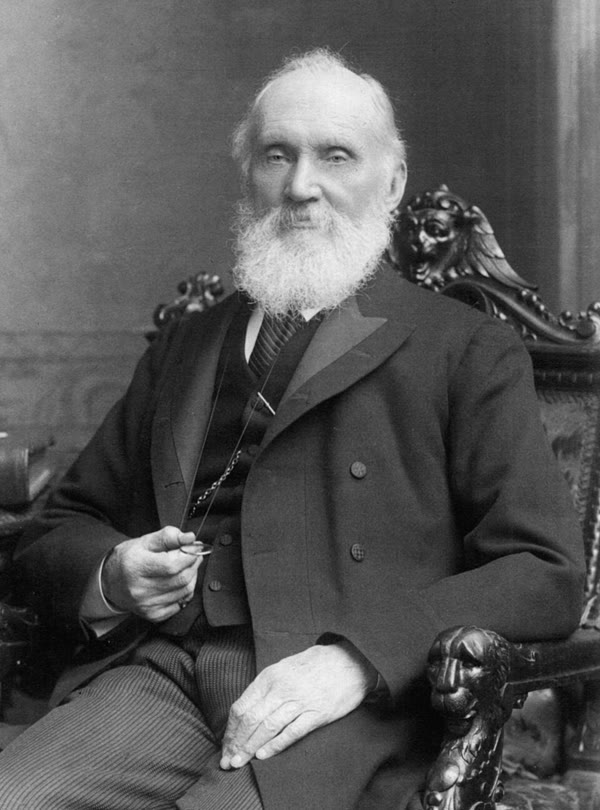
\includegraphics[height=5.2cm]{images/book2/g12-kelvin-1906.jpg}

{\small विलियम थॉमसन, लॉर्ड केल्विन, 1906 में। फ़ोटो रसेल ऐंड संस,
लंदन (स्मिथसोनियन संस्थान पुस्तकालय, कोई ज्ञात कॉपीराइट प्रतिबंध नहीं)।}
\end{omfigure}
% ledger: photo:g12-kelvin

\begin{recall}
सापेक्ष काल-निर्धारण चट्टानों और घटनाओं को क्रम में रखता है; निरपेक्ष आयु वर्षों की एक संख्या
है (पुस्तक 1, कक्षा 7)। कोई रेडियोधर्मी समस्थानिक, जनक, यादृच्छिक रूप से एक
संतति समस्थानिक में क्षयित होता है: बचे हुए जनक परमाणुओं की संख्या $N$
$N = N_0\,e^{-\lambda t}$ के अनुसार घटती है, जहाँ $\lambda$ क्षय-स्थिरांक है, और
हर अर्ध-आयु $T = \ln 2/\lambda$ में आधी होती है (भौतिकी की पुस्तकें)। सबसे पुराने ज्ञात
खनिज, पश्चिमी ऑस्ट्रेलिया के ज़र्कॉन, 4.4 अरब वर्ष पुराने हैं
(\cref{ch:g12:continental-crust})। पृथ्वी वह ऊष्मा भी खोती है जिसे रेडियोधर्मिता
बनाती रहती है, और उसके प्रावार में संवहन होता है (\cref{ch:g12:internal-heat})।
\end{recall}
% ledger: wilde01:zircon

\section{अनुमानों का एक इतिहास}

रेडियोधर्मिता से पहले, \omterm{def:g12:age-of-the-earth:age}{पृथ्वी की आयु} का हर अनुमान किसी ऐसी प्रक्रिया पर टिका था
जिसकी दर ज्ञात मानी गई थी।

\begin{center}
\small
\begin{tabular}{|p{0.19\linewidth}|p{0.42\linewidth}|p{0.25\linewidth}|}
\hline
कौन, कब & विधि और उसकी मान्यता & अनुमान \\
\hline
फ़िलिप्स, 1860 & अवसादी परतों की मोटाई को निक्षेपण की एक दर से भाग; स्थिर दर मानता है & 38 से 96 मिलियन वर्ष \\
केल्विन, 1862 & पिघली पृथ्वी का केवल चालन द्वारा शीतलन, भीतर ऊष्मा के किसी स्रोत के बिना & 20 से 400 मिलियन वर्ष \\
जी॰\,एच॰~डार्विन & चंद्रमा के पृथ्वी से अलग होने के बाद का समय, ज्वार द्वारा उनकी गतियों के धीमे होने से & कम से कम 56 मिलियन वर्ष \\
जॉली, 1899 & नदियों द्वारा समुद्र तक ले जाया गया नमक, वार्षिक आपूर्ति से भाग; स्थिर आपूर्ति मानता है और कोई नमक हटता नहीं & 80 से 100 मिलियन वर्ष \\
\hline
\end{tabular}
\end{center}
% ledger: holmes13:estimates

\begin{history}[केल्विन की लुप्त ऊष्मा]
1903 में पियरे क्यूरी और अल्बेर लाबोर्द ने दिखाया कि रेडियम ऊष्मा छोड़ता है,
और कई वैज्ञानिकों ने जल्द ही तर्क दिया कि यह ऊष्मा केल्विन के निष्कर्ष को
उलट देती है। एक वर्ष बाद अर्नेस्ट रदरफ़ोर्ड ने, जब श्रोताओं में केल्विन बैठे थे,
व्याख्यान देते हुए उन्हें याद दिलाया कि उन्होंने \omterm{def:g12:age-of-the-earth:age}{पृथ्वी की आयु} की सीमा
``इस शर्त पर कि ऊष्मा का कोई नया स्रोत न खोजा जाए'' बाँधी थी। रेडियोधर्मिता
वही स्रोत लगती थी। फिर भी यह केल्विन की मुख्य त्रुटि नहीं थी: पृथ्वी के शीतलन को सबसे अधिक
लंबा करने वाला \omterm{def:g12:internal-heat:convection}{प्रावार संवहन} है, जो ऊपरी प्रावार को गरम और भूपर्पटी में
प्रवणता को केवल चालन की अपेक्षा कहीं अधिक समय तक ऊँचा रखता है।
\end{history}
% ledger: england:kelvin (Book 3 row)

रेडियोधर्मिता ने एक घड़ी भी दी। 1907 में बर्ट्रम बोल्टवुड ने दिखाया कि
एक ही आयु के यूरेनियम खनिजों में यूरेनियम के हर ग्राम के लिए सीसे की मात्रा
समान होती है: सीसा यूरेनियम से बनता है। 1913 तक आर्थर होम्स
लिख सके कि काल-निर्धारित सबसे पुरानी चट्टानें \num{1600} मिलियन वर्ष पुरानी थीं, और
1927 में उन्होंने \omterm{def:g12:age-of-the-earth:age}{पृथ्वी की आयु} 1.6 और 3.0 अरब वर्ष के बीच रखी। 1956 में क्लेयर
पैटरसन ने 4.55 अरब वर्ष मापे। आज का मान 4.54 अरब वर्ष है,
एक प्रतिशत के भीतर।
% ledger: holmes13:estimates, holmes27:age, patterson56:table, usgs:age-earth (Book 1 row)

\begin{omfigure}
\begin{tikzpicture}
\begin{axis}[omrecord, width=0.78\linewidth, height=6.2cm, ymode=log, xmin=1840, xmax=2040,
  ymin=1e7, ymax=2e10, xlabel={अनुमान का वर्ष}, ylabel={पृथ्वी की अनुमानित आयु (वर्ष)},
  xtick={1850,1875,...,2025}, x tick label style={/pgf/number format/.cd, set thousands separator={}},
  ytick={1e7,1e8,1e9,1e10}, ymajorgrids=true, xmajorgrids=false]
% computed in figdata/grade-12/isochrons.py; ledger: holmes13:estimates, holmes27:age, patterson56:table, usgs:age-earth (Book 1 row)
\addplot[omDef, only marks, mark=*, mark size=1.8pt, error bars/.cd, y dir=both, y explicit]
  table[x=year, y=mid, y error minus expr=\thisrow{mid}-\thisrow{lo}, y error plus expr=\thisrow{hi}-\thisrow{mid}]
  {figdata/out/grade-12-isochrons-history.dat};
\addplot[omThm, densely dashed, domain=1840:2040, samples=2] {4.54e9};
\coordinate (k62) at (axis cs:1862,2.4e8);
\coordinate (k97) at (axis cs:1897,2.8e7);
\coordinate (jol) at (axis cs:1899,1e8);
\coordinate (h11) at (axis cs:1919,1.3e9);
\coordinate (pat) at (axis cs:1956,4.55e9);
\coordinate (now) at (axis cs:1845,4.54e9);
\end{axis}
\node[font=\scriptsize, anchor=west] at ([xshift=4pt]k62) {केल्विन 1862};
\node[font=\scriptsize, anchor=east] at ([xshift=-4pt]k97) {केल्विन 1897};
\node[font=\scriptsize, anchor=west] at ([xshift=4pt]jol) {जॉली};
\node[font=\scriptsize, anchor=north] at (h11) {होम्स};
\node[font=\scriptsize, anchor=north west] at ([xshift=2pt, yshift=-3pt]pat) {पैटरसन};
\node[font=\scriptsize, text=omThm, anchor=south west] at (now) {आज, 4.54 अरब वर्ष};
\end{tikzpicture}

{\small \omterm{def:g12:age-of-the-earth:age}{पृथ्वी की आयु} के अनुमान, जिस वर्ष वे किए गए उसके सापेक्ष,
लघुगणकीय पैमाने पर; पट्टियाँ हर लेखक द्वारा दिए गए परास को दिखाती हैं। होम्स का 1913 वाला
बिंदु तब काल-निर्धारित सबसे पुरानी चट्टानों की आयु है, एक न्यूनतम। स्रोत: होम्स
(1913, 1927); पैटरसन (1956); अमेरिकी भूवैज्ञानिक सर्वेक्षण।}
\end{omfigure}

\section{एक रेडियोधर्मी घड़ी}

रेडियोधर्मी घड़ी तभी काम करती है जब उसके चलना शुरू करने के बाद से उसमें न कुछ जोड़ा गया हो,
न उससे कुछ निकाला गया हो।

\begin{definition}[बंद तंत्र]\label{def:g12:age-of-the-earth:closed-system}
कोई चट्टान या खनिज किसी जनक समस्थानिक और उसकी संतति के लिए \emph{बंद तंत्र}\index{बंद तंत्र}
है, यदि उसकी घड़ी चलना शुरू होने के क्षण से,
जनक या संतति का कोई भी परमाणु उसमें न आया हो और न उससे गया हो, सिवाय
जनक के संतति में क्षय द्वारा।
\end{definition}
% ledger: tulane:radiometric

किसी खनिज के लिए घड़ी तब शुरू होती है जब वह किसी मैग्मा से क्रिस्टलित होता है, या अधिक
ठीक-ठीक, जब वह इतना ठंडा हो चुका होता है कि परमाणु उसमें आना-जाना बंद कर दें।
गरम होना, कोई गरम
तरल या अपक्षय तंत्र को फिर से खोल सकते हैं, और तब मापी गई आयु
ग़लत होती है, या उस बाद की घटना की तिथि बताती है।
% ledger: tulane:radiometric

किसी \omterm{def:g12:age-of-the-earth:closed-system}{बंद तंत्र} में संतति परमाणुओं को गिनने से आयु मिलती है, बशर्ते यह
ज्ञात हो कि शुरुआत में कितने थे। प्रायः यह ज्ञात नहीं होता। रुबिडियम-87
स्ट्रॉन्शियम-87 में क्षयित होता है, पर हर खनिज ने बनते समय कुछ स्ट्रॉन्शियम-87
भी ग्रहण किया था। \omterm{def:g12:age-of-the-earth:isochron}{समकालरेखा} विधि एक चट्टान के कई खनिजों को मापकर
इस कठिनाई से बचती है।

\section{समकालरेखा}

स्ट्रॉन्शियम का एक समस्थानिक, स्ट्रॉन्शियम-86, स्थायी है और किसी
क्षय से नहीं बनता: \omterm{def:g12:age-of-the-earth:closed-system}{बंद तंत्र} में उसकी संख्या वही रहती है, और वह एक
मापदंड का काम करता है। समस्थानिक अनुपात $^{87}\mathrm{Sr}/^{86}\mathrm{Sr}$ और
$^{87}\mathrm{Rb}/^{86}\mathrm{Sr}$ वे हैं जिन्हें द्रव्यमान स्पेक्ट्रममापी मापता है।

\begin{theorem}[समकालरेखा समीकरण]\label{thm:g12:age-of-the-earth:isochron}
किसी ऐसे खनिज में जो समय $t$ से \omterm{def:g12:age-of-the-earth:closed-system}{बंद तंत्र} रहा है,
\[
  \left(\frac{^{87}\mathrm{Sr}}{^{86}\mathrm{Sr}}\right)_{\text{आज}}
  = \left(\frac{^{87}\mathrm{Sr}}{^{86}\mathrm{Sr}}\right)_{0}
  + \left(\frac{^{87}\mathrm{Rb}}{^{86}\mathrm{Sr}}\right)_{\text{आज}}
  \left(e^{\lambda t} - 1\right),
\]
जहाँ सूचकांक 0 उस मान को दर्शाता है जब घड़ी चलनी शुरू हुई, और $\lambda$
रुबिडियम-87 का क्षय-स्थिरांक है।
\end{theorem}

\begin{proof}
मान लीजिए $P$ अभी रुबिडियम-87 परमाणुओं की संख्या है और $P_0$ वह जब घड़ी
चलनी शुरू हुई। क्षय-नियम से $P = P_0\,e^{-\lambda t}$, इसलिए $P_0 = P\,e^{\lambda t}$,
और क्षयित हुए परमाणुओं की संख्या $P_0 - P = P\,(e^{\lambda t}-1)$ है।
\omterm{def:g12:age-of-the-earth:closed-system}{बंद तंत्र} में उनमें से हर एक स्ट्रॉन्शियम-87 का एक परमाणु बन गया है, जो
शुरुआत में मौजूद $D_0$ परमाणुओं में जुड़ जाता है: $D = D_0 + P\,(e^{\lambda
t}-1)$। स्ट्रॉन्शियम-86 परमाणुओं की संख्या से, जो बदली नहीं है, भाग देने पर
समीकरण मिलता है।
\end{proof}
% ledger: tulane:radiometric

किसी ग्रेनाइट के खनिज एक ही मैग्मा से क्रिस्टलित हुए, इसलिए उन सबने
एक ही अनुपात $(^{87}\mathrm{Sr}/^{86}\mathrm{Sr})_0$ से शुरुआत की। पर उन्होंने
रुबिडियम की बहुत भिन्न मात्राएँ ग्रहण कीं। उन सबका $t$ और प्रारंभिक अनुपात एक ही है, इसलिए
समीकरण कहता है कि उनके बिंदु एक ही सीधी रेखा पर पड़ते हैं।

\begin{definition}[समकालरेखा]\label{def:g12:age-of-the-earth:isochron}
\emph{समकालरेखा}\index{समकालरेखा} वह सीधी रेखा है जिस पर उन
खनिजों या चट्टानों के बिंदु पड़ते हैं जो एक ही समय पर एक ही
स्रोत से बने और तब से \omterm{def:g12:age-of-the-earth:closed-system}{बंद तंत्र} रहे हैं, जब संतति और
स्थायी समस्थानिक के अनुपात को जनक और स्थायी समस्थानिक के अनुपात के सापेक्ष आलेखित किया जाता है। उसका
ढाल उनकी आयु देता है, और वह बिंदु जहाँ वह ऊर्ध्वाधर अक्ष से मिलती है,
उनका प्रारंभिक अनुपात देता है।
\end{definition}
% ledger: tulane:radiometric

\begin{proposition}[ढाल से आयु]\label{prop:g12:age-of-the-earth:slope}
यदि किसी \omterm{def:g12:age-of-the-earth:isochron}{समकालरेखा} का ढाल $m$ है, तो आयु है
\[
  t = \frac{\ln(1+m)}{\lambda}.
\]
\end{proposition}

\begin{proof}
\omterm{def:g12:age-of-the-earth:isochron}{समकालरेखा} समीकरण से तुलना करने पर $m = e^{\lambda t} - 1$, इसलिए
$e^{\lambda t} = 1 + m$, $\lambda t = \ln(1+m)$, और $t = \ln(1+m)/\lambda$।
\end{proof}

रुबिडियम-87 के लिए $\lambda = \num{1.3972e-11}$ प्रति वर्ष, यानी
$\ln 2/\lambda \approx 49.6$ अरब वर्ष की अर्ध-आयु: \omterm{def:g12:age-of-the-earth:age}{पृथ्वी की आयु} के दस गुने से
भी अधिक।
% ledger: villa22:rb87

\begin{method}[समकालरेखा से किसी चट्टान का काल-निर्धारण]\label{met:g12:age-of-the-earth:isochron}
\begin{enumerate}
  \item चट्टान के कई खनिज अलग कीजिए (या उसके कई नमूने
        लीजिए) जिनमें रुबिडियम की मात्राएँ भिन्न हों।
  \item हर एक में अनुपात $^{87}\mathrm{Rb}/^{86}\mathrm{Sr}$ ($x$)
        और $^{87}\mathrm{Sr}/^{86}\mathrm{Sr}$ ($y$) मापिए।
  \item $y$ को $x$ के सापेक्ष आलेखित कीजिए और जाँचिए कि बिंदु एक सीधी
        रेखा पर पड़ते हैं: यदि कोई नहीं पड़ता, तो वह नमूना \omterm{def:g12:age-of-the-earth:closed-system}{बंद तंत्र} नहीं था।
  \item रेखा का ढाल $m$ लीजिए, और $t = \ln(1+m)/\lambda$ परिकलित कीजिए।
  \item जहाँ रेखा ऊर्ध्वाधर अक्ष से मिलती है, वहाँ प्रारंभिक अनुपात पढ़िए।
\end{enumerate}
\end{method}

\begin{example}[वार्डन ग्रेनाइट]\label{ex:g12:age-of-the-earth:varden}
वार्डन पहाड़ियों का ग्रेनाइट, श्रृंखला का कल्पित क्षेत्र, ये
अनुपात देता है (अभ्यास के आँकड़े):
\begin{center}
\small
\begin{tabular}{|l|c|c|}
\hline
नमूना & $^{87}\mathrm{Rb}/^{86}\mathrm{Sr}$ & $^{87}\mathrm{Sr}/^{86}\mathrm{Sr}$ \\
\hline
प्लेजियोक्लेज़ & 0.35 & 0.70952 \\
हॉर्नब्लेंड  & 1.20 & 0.71321 \\
पूर्ण चट्टान  & 3.10 & 0.72146 \\
K-फ़ेल्डस्पार  & 6.40 & 0.73578 \\
बायोटाइट     & 24.0 & 0.81218 \\
\hline
\end{tabular}
\end{center}
प्लेजियोक्लेज़ और बायोटाइट से होकर ढाल है
$m = (0.81218 - 0.70952)/(24.0 - 0.35) \approx 0.004341$। तब
$t = \ln(1.004341)/\num{1.3972e-11} \approx \num{3.10e8}$ वर्ष:
ग्रेनाइट 310 मिलियन वर्ष पुराना है। रेखा ऊर्ध्वाधर अक्ष से
$0.70952 - 0.35 \times 0.004341 \approx 0.7080$ पर मिलती है, यही प्रारंभिक अनुपात है।
\end{example}
% values: granite_age_Ma 310.0, granite_intercept 0.70800 (isochrons.py)

\begin{omfigure}
\begin{tikzpicture}
\begin{axis}[omrecord, width=0.7\linewidth, height=6cm, xmin=0, xmax=26, ymin=0.695, ymax=0.82, ytick={0.70,0.72,...,0.82},
  xlabel={$^{87}\mathrm{Rb}/^{86}\mathrm{Sr}$}, ylabel={$^{87}\mathrm{Sr}/^{86}\mathrm{Sr}$},
  y tick label style={/pgf/number format/.cd, fixed, fixed zerofill, precision=2}]
% computed in figdata/grade-12/isochrons.py (exercise data, Varden granite 310 Ma); ledger: villa22:rb87
\addplot[omDef, line width=0.9pt] table[x=x, y=y] {figdata/out/grade-12-isochrons-graniteln.dat};
\addplot[omThm, only marks, mark=*, mark size=2pt] table[x=rbsr, y=srsr] {figdata/out/grade-12-isochrons-granite.dat};
\addplot[black!60, densely dotted, domain=0:26, samples=2] {0.7080};
\coordinate (pl) at (axis cs:0.35,0.70952);
\coordinate (hb) at (axis cs:1.2,0.71321);
\coordinate (wr) at (axis cs:3.1,0.72146);
\coordinate (kf) at (axis cs:6.4,0.73578);
\coordinate (bt) at (axis cs:24,0.81218);
\coordinate (sl) at (axis cs:12,0.762);
\coordinate (in) at (axis cs:9,0.7082);
\coordinate (plhb) at (axis cs:0.6,0.737);
\coordinate (plhbpt) at (axis cs:0.9,0.7125);
\end{axis}
\node[font=\scriptsize, anchor=north west] at ([xshift=1pt]wr) {पूर्ण चट्टान};
\node[font=\scriptsize, anchor=north west] at ([xshift=1pt]kf) {K-फ़ेल्डस्पार};
\node[font=\scriptsize, anchor=east] at ([xshift=-3pt]bt) {बायोटाइट};
\node[font=\scriptsize, anchor=south west, align=left, inner sep=1pt] (plhblab) at (plhb) {प्लेजियोक्लेज़,\\हॉर्नब्लेंड};
\draw[black!60, line width=0.4pt] (plhblab.south) -- (plhbpt);
\node[font=\scriptsize, text=omDef, anchor=south east] at (sl) {ढाल $0.004341$: 310 मिलियन वर्ष};
\node[font=\scriptsize, text=black!70, anchor=south west] at (in) {प्रारंभिक अनुपात 0.7080 (समय 0)};
\end{tikzpicture}

{\small वार्डन ग्रेनाइट की रुबिडियम--स्ट्रॉन्शियम \omterm{def:g12:age-of-the-earth:isochron}{समकालरेखा} (अभ्यास के
आँकड़े)। जब ग्रेनाइट बना, तब उसके सभी खनिज बिंदुकित
क्षैतिज रेखा पर थे; तब से हर एक अपने रुबिडियम के अनुपात में ऊपर उठा है, और
अब वे ठोस रेखा पर हैं।}
\end{omfigure}

\begin{inthelab}[परमाणुओं को तौलना]
अनुपात द्रव्यमान स्पेक्ट्रममापी से मापे जाते हैं। किसी खनिज के कुछ
मिलीग्राम अम्ल में घोले जाते हैं, और स्ट्रॉन्शियम को रसायन द्वारा
रुबिडियम से अलग किया जाता है, क्योंकि अन्यथा द्रव्यमान 87 के दोनों समस्थानिक
एक साथ गिने जाते। स्ट्रॉन्शियम, धातु के एक तंतु पर जमाकर निर्वात में गरम
किए जाने पर, आयन छोड़ता है; एक विद्युत क्षेत्र उन्हें तेज़ करता है और एक चुंबक
उनके पथ मोड़ता है, हल्के आयनों को भारी आयनों से अधिक, जिससे हर
समस्थानिक अपने संग्राहक तक पहुँचता है। उनकी धाराएँ अनुपात देती हैं।
\end{inthelab}

\begin{omfigure}
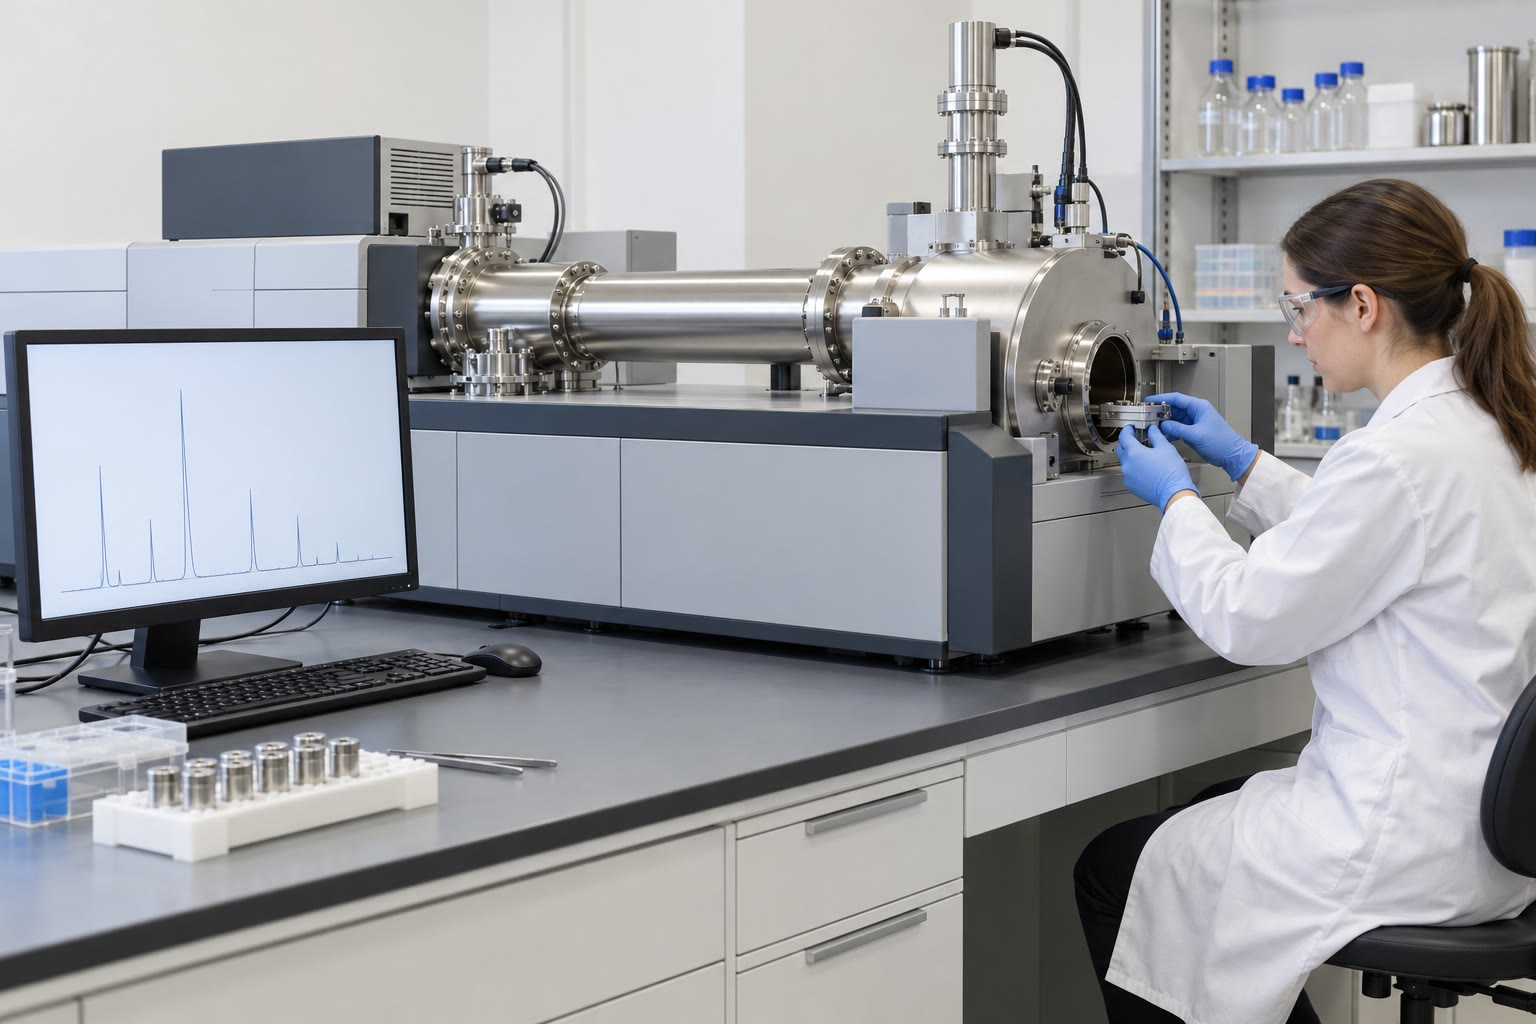
\includegraphics[width=0.66\linewidth]{images/book2/ai/g12-mass-spectrometer-lab.jpg}

{\small प्रयोगशाला में एक द्रव्यमान स्पेक्ट्रममापी: स्रोत वाले सिरे पर एक नमूना
लगाया जा रहा है। एआई-जनित चित्रण।}
\end{omfigure}

प्रारंभिक अनुपात इसका भी सुराग है कि मैग्मा कहाँ से आया। प्रावार के पिघलने पर
रुबिडियम गलित को पसंद करता है, इसलिए युगों में वह
\omterm{def:g12:continental-crust:continental-crust}{महाद्वीपीय भूपर्पटी} में सांद्रित होता गया है, जिसने इसलिए अधिक
स्ट्रॉन्शियम-87 बनाया है: भूपर्पटी की चट्टानों का $^{87}\mathrm{Sr}/^{86}\mathrm{Sr}$
प्रावार की चट्टानों से अधिक होता है। पिघली भूपर्पटी से बना मैग्मा वह ऊँचा अनुपात विरासत में पाता है।
% ledger: tulane:radiometric

\section{पृथ्वी की आयु}

पृथ्वी पर कोई चट्टान पृथ्वी के आरंभ तक नहीं जाती: सबसे पुरानी ज्ञात चट्टान,
अकास्टा नाइस, 4.03 अरब वर्ष पुरानी है, और सबसे पुराने ज़र्कॉन 4.4
अरब। तब से सतह पिघली, अपरदित हुई और पुनर्चक्रित हुई है। स्वयं पृथ्वी का
काल-निर्धारण उल्कापिंडों से आता है, उन छोटे पिंडों के टुकड़े
जो ग्रहों के साथ बने और जिनमें से कुछ तब से
\omterm{def:g12:age-of-the-earth:closed-system}{बंद तंत्र} बने रहे हैं।
% ledger: bowring99:acasta, wilde01:zircon, usgs:age-earth (Book 1 row)

\begin{definition}[पृथ्वी की आयु]\label{def:g12:age-of-the-earth:age}
\emph{पृथ्वी की आयु}\index{पृथ्वी की आयु} वह समय है जो
सौर मंडल के जन्म के समय छोटे पिंडों की अभिवृद्धि से पृथ्वी के बनने के बाद से बीता है।
उल्कापिंडों से रेडियोमितीय काल-निर्धारण द्वारा मापी गई यह
\num{4.54} अरब वर्ष है, एक प्रतिशत के भीतर।
\end{definition}
% ledger: usgs:age-earth (Book 1 row)

1956 में क्लेयर पैटरसन ने तीन पथरीले
उल्कापिंडों और दो लौह उल्कापिंडों में सीसे के समस्थानिक मापे। सीसे के दो समस्थानिक
यूरेनियम के क्षय से बनते हैं, सीसा-206 यूरेनियम-238 से और सीसा-207 यूरेनियम-235 से,
जबकि सीसा-204 किसी क्षय से नहीं बनता। स्ट्रॉन्शियम की तरह, एक ही समय पर बने
उल्कापिंडों के बिंदु एक सीधी रेखा पर पड़ते हैं, जब
$^{207}\mathrm{Pb}/^{204}\mathrm{Pb}$ को
$^{206}\mathrm{Pb}/^{204}\mathrm{Pb}$ के सापेक्ष आलेखित किया जाता है। एरिज़ोना के कैनियन डियाब्लो
लौह उल्कापिंड में लगभग कोई यूरेनियम नहीं है: बनने के बाद से उसका सीसा नहीं बदला है,
और वह रेखा के निचले सिरे को चिह्नित करता है, वह सीसा जिससे सौर मंडल ने शुरुआत की।
% ledger: patterson56:table, patterson56:constants, usgs:age-earth (Book 1 row: Canyon Diablo troilite)

\begin{omfigure}
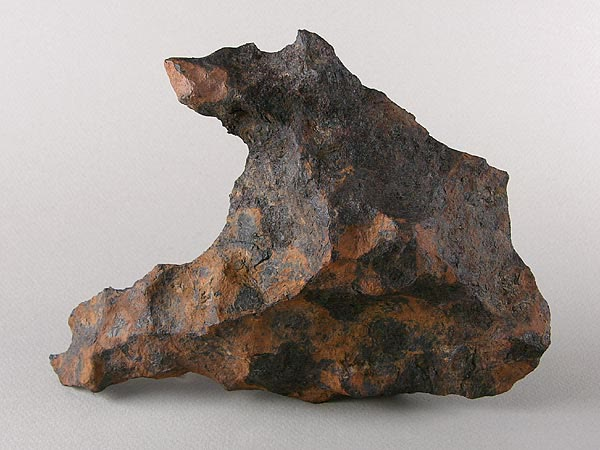
\includegraphics[height=4.2cm]{images/book2/g12-canyon-diablo-meteorite.jpg}

{\small कैनियन डियाब्लो लौह उल्कापिंड का एक टुकड़ा, \qty{2641}{g}।
फ़ोटो जेफ़्री नॉटकिन, CC~BY-SA~2.5 (विकिमीडिया कॉमन्स)।}
\end{omfigure}
% ledger: photo:g12-canyon-diablo

सीसे के लिए ढाल $m$ दोनों यूरेनियम समस्थानिकों के माध्यम से आयु पर निर्भर है; यह
संबंध यहाँ मान लिया गया है। पैटरसन द्वारा उपयोग किए गए स्थिरांकों के साथ,
\[
  m = \frac{1}{137.8}\,\frac{e^{\lambda_{235}t}-1}{e^{\lambda_{238}t}-1},
  \qquad \lambda_{235} = \num{9.72e-10},\ \lambda_{238} = \num{1.537e-10}
  \text{ प्रति वर्ष},
\]
जो यह देता है:
\begin{center}
\small
\begin{tabular}{|l|c|c|c|c|c|c|}
\hline
आयु (अरब वर्ष) & 4.40 & 4.45 & 4.50 & 4.55 & 4.60 & 4.65 \\
ढाल $m$ & 0.533 & 0.551 & 0.570 & 0.590 & 0.610 & 0.632 \\
\hline
\end{tabular}
\end{center}
% ledger: patterson56:constants
% values: pb_slope at 4.40-4.65 Ga (isochrons.py pb_slope)

\begin{omfigure}
\begin{tikzpicture}
\begin{axis}[omrecord, width=0.72\linewidth, height=6cm, xmin=0, xmax=56, ymin=0, ymax=40,
  xlabel={$^{206}\mathrm{Pb}/^{204}\mathrm{Pb}$}, ylabel={$^{207}\mathrm{Pb}/^{204}\mathrm{Pb}$}]
% computed in figdata/grade-12/isochrons.py; ledger: patterson56:table
\addplot[omDef, line width=0.9pt] table[x=x, y=y] {figdata/out/grade-12-isochrons-pbln.dat};
\addplot[omThm, only marks, mark=*, mark size=2pt] table[x=r206, y=r207, restrict expr to domain={\thisrow{idx}}{1:5}] {figdata/out/grade-12-isochrons-pbpb.dat};
\addplot[black, only marks, mark=o, mark size=2.6pt, line width=0.8pt] table[x=r206, y=r207, restrict expr to domain={\thisrow{idx}}{6:6}] {figdata/out/grade-12-isochrons-pbpb.dat};
\coordinate (nl) at (axis cs:50.28,34.86);
\coordinate (fc) at (axis cs:19.48,15.76);
\coordinate (cd) at (axis cs:9.5,10.36);
\coordinate (sed) at (axis cs:19.0,15.5);
\coordinate (sl) at (axis cs:30,25);
\end{axis}
\node[font=\scriptsize, anchor=north west] at ([xshift=2pt]nl) {नुएवो लारेदो};
\node[font=\scriptsize, anchor=north west, align=left] at ([xshift=4pt, yshift=-2pt]fc) {फ़ॉरेस्ट सिटी, मोडॉक;\\महासागरीय अवसाद (वृत्त)};
\node[font=\scriptsize, anchor=north west, align=left] at ([xshift=3pt, yshift=-3pt]cd) {कैनियन डियाब्लो, हेनबरी (लौह)};
\node[font=\scriptsize, text=omDef, anchor=south east] at (sl) {ढाल 0.603: लगभग 4.6 अरब वर्ष};
\end{tikzpicture}

{\small पैटरसन की सीसा \omterm{def:g12:age-of-the-earth:isochron}{समकालरेखा}: पाँचों उल्कापिंड एक रेखा पर पड़ते हैं, और
लगभग उसी पर एक आधुनिक महासागरीय अवसाद का सीसा भी, जो पृथ्वी का प्रतिनिधि है।
स्रोत: पैटरसन (1956), तालिका~1।}
\end{omfigure}
% values: pb_slope 0.6026, pb_age_Ga 4.58, sediment_residual -0.39 (isochrons.py)

पाँचों बिंदुओं से होकर खींची गई रेखा का ढाल लगभग 0.603 है, तालिका में
4.55 और 4.60 अरब वर्ष के ढालों के बीच। पैटरसन का अपना
परिणाम, मापनों और क्षय-स्थिरांकों की त्रुटियों को ध्यान में रखते हुए,
4.55 अरब वर्ष था, 0.07 कम या अधिक। फिर उन्होंने एक आधुनिक महासागरीय अवसाद का सीसा मापा, जो
पृथ्वी की भूपर्पटी के एक विशाल पिंड का सीसा मिलाता है: वह उसी रेखा पर पड़ता है।
पृथ्वी का सीसा उल्कापिंडों के सीसे की तरह, उतने ही समय में, विकसित हुआ है:
पृथ्वी उतनी ही पुरानी है जितने वे।
% ledger: patterson56:table

तब से सैकड़ों मापनों ने इसकी पुष्टि की है। उल्कापिंड
4.53 से 4.58 अरब वर्ष तक की आयु देते हैं, और सौर मंडल के सबसे पुराने ठोस,
कुछ उल्कापिंडों में मिलने वाले कैल्सियम और ऐलुमिनियम से समृद्ध छोटे अंतर्वेश,
\num{4567.30} मिलियन वर्ष पहले बने, 0.16 कम या अधिक। पृथ्वी
बाद में ऐसे पदार्थ से बनी, इसीलिए उसकी आयु, 4.54 अरब वर्ष, उनकी आयु से
थोड़ी कम है।
% ledger: usgs:age-earth (Book 1 row), connelly12:cai

\section{अभ्यास}

\begin{exercise}[$\star$]\label{exo:g12:age-of-the-earth:1}
शब्द बताइए: (a) ऐसा खनिज जिसमें उसकी घड़ी शुरू होने के बाद से कोई जनक या संतति परमाणु
न आया हो, न उससे गया हो; (b) वह सीधी रेखा जिस पर एक ही आयु और एक ही स्रोत के
खनिज पड़ते हैं; (c) अभिवृद्धि द्वारा पृथ्वी के बनने के बाद से बीता
समय।
\end{exercise}

\begin{exercise}[$\star$]\label{exo:g12:age-of-the-earth:2}
वार्डन ग्रेनाइट की तालिका का उपयोग करके उसके पाँच नमूनों को उनके
रुबिडियम-87 और स्ट्रॉन्शियम-86 के अनुपात के क्रम में, सबसे कम से शुरू करके, रखिए। उनमें से कौन
\omterm{def:g12:age-of-the-earth:isochron}{समकालरेखा} पर सबसे ऊँचा पड़ता है, और उसने सबसे अधिक स्ट्रॉन्शियम-87 क्यों बनाया है?
\end{exercise}

\begin{exercise}[$\star$]\label{exo:g12:age-of-the-earth:3}
रुबिडियम-87 की अर्ध-आयु उसके क्षय-स्थिरांक,
प्रति वर्ष \num{1.3972e-11}, से परिकलित कीजिए। यह \omterm{def:g12:age-of-the-earth:age}{पृथ्वी की आयु} का कितना गुना है?
\end{exercise}

\begin{exercise}[$\star$]\label{exo:g12:age-of-the-earth:4}
रुबिडियम-87 के लिए $e^{\lambda t} - 1$ परिकलित कीजिए, $t = 310$ मिलियन वर्ष और
$t = 480$ मिलियन वर्ष के लिए।
\end{exercise}

\begin{exercise}[$\star$]\label{exo:g12:age-of-the-earth:5}
फ़िलिप्स, होम्स (1927), जॉली, केल्विन
(1862) और पैटरसन के अनुमानों को तिथि के क्रम में रखिए। पृथ्वी की आज की आयु जॉली के
अनुमान के ऊपरी सिरे का कितना गुना है?
\end{exercise}

\begin{exercise}[$\star\star$]\label{exo:g12:age-of-the-earth:6}
वार्डन ग्रेनाइट (310 मिलियन वर्ष, प्रारंभिक अनुपात 0.7080) के एक खनिज का
$^{87}\mathrm{Rb}/^{86}\mathrm{Sr} = 10.0$ है। आज उसका
$^{87}\mathrm{Sr}/^{86}\mathrm{Sr}$ क्या है? ग्रेनाइट के बनने के समय यह क्या
था?
\end{exercise}

\begin{exercise}[$\star\star$]\label{exo:g12:age-of-the-earth:7}
वार्डन शिस्ट के चार नमूने $(x, y)$ = (0.90, 0.71806),
(2.60, 0.72950), (5.10, 0.74632) और (9.40, 0.77525) देते हैं, जहाँ $x =
{}^{87}\mathrm{Rb}/^{86}\mathrm{Sr}$ और $y = {}^{87}\mathrm{Sr}/^{86}\mathrm{Sr}$।
(1) पहले और अंतिम नमूनों से ढाल और आयु परिकलित कीजिए।
(2) जाँचिए कि बीच के दोनों नमूने उसी रेखा पर पड़ते हैं। (3) क्या यह
परिणाम ग्रेनाइट के 310 मिलियन वर्ष और अनुप्रस्थ काट के सिद्धांत से
संगत है?
\end{exercise}

\begin{exercise}[$\star\star$]\label{exo:g12:age-of-the-earth:8}
जिस चट्टान के सभी खनिजों में रुबिडियम और स्ट्रॉन्शियम का अनुपात एक ही हो, वह
\omterm{def:g12:age-of-the-earth:isochron}{समकालरेखा} क्यों नहीं देती? वार्डन ग्रेनाइट में बायोटाइट दूसरे खनिजों की अपेक्षा
ढाल को बेहतर क्यों तय करता है?
\end{exercise}

\begin{exercise}[$\star\star$]\label{exo:g12:age-of-the-earth:9}
वार्डन ग्रेनाइट के बनने के बहुत बाद, एक गरम तरल के कारण उसके बायोटाइट ने
अपने स्ट्रॉन्शियम-87 का कुछ भाग खो दिया। (1) \omterm{def:g12:age-of-the-earth:isochron}{समकालरेखा} आरेख पर उसका बिंदु कहाँ खिसकता है?
(2) तब अकेले बायोटाइट और प्लेजियोक्लेज़ कौन-सी आयु देंगे: बहुत अधिक या
बहुत कम? (3) \omterm{def:g12:age-of-the-earth:isochron}{समकालरेखा} विधि इस समस्या को कैसे प्रकट करती है?
\end{exercise}

\begin{exercise}[$\star\star$]\label{exo:g12:age-of-the-earth:10}
(1) \omterm{def:g12:age-of-the-earth:age}{पृथ्वी की आयु} केल्विन के 96 मिलियन वर्ष से कितने गुना अधिक
है? (2) जॉली ने माना कि नदियाँ समुद्र तक नमक स्थिर
दर से लाती हैं और उसमें से कुछ भी समुद्र से नहीं निकलता। इनमें से कौन-सी मान्यता, ग़लत होने पर,
उनकी आयु को बहुत कम कर देती है, और क्यों?
\end{exercise}

\begin{exercise}[$\star\star$]\label{exo:g12:age-of-the-earth:11}
कैनियन डियाब्लो (9.46, 10.34) और नुएवो लारेदो
(50.28, 34.86) के लिए पैटरसन के मानों का उपयोग करके, दोनों उल्कापिंडों से होकर जाती रेखा का ढाल
परिकलित कीजिए, और ढालों की तालिका से आयु पढ़िए।
\end{exercise}

\begin{exercise}[$\star\star\star$]\label{exo:g12:age-of-the-earth:12}
वार्डन क्षेत्र का एक बेसाल्ट, वह भी 310 मिलियन वर्ष पुराना, का प्रारंभिक
अनुपात 0.7035 है, जबकि ग्रेनाइट का 0.7080। (1) कौन-सी चट्टान पिघले प्रावार से
आई होने की अधिक संभावना रखती है, और कौन-सी पिघली भूपर्पटी से? (2) रुबिडियम के बारे में
आप जो जानते हैं, उससे कारण समझाइए। (3) क्या दोनों एक ही मैग्मा से
क्रिस्टलित हो सकती थीं?
\end{exercise}

\begin{exercise}[$\star\star\star$]\label{exo:g12:age-of-the-earth:13}
(1) पृथ्वी के बनने के समय मौजूद रुबिडियम-87 का कितना अंश आज
बचा है? और यूरेनियम-238 का (अर्ध-आयु 4.47 अरब वर्ष)? (2) एक मिलियन वर्ष पुरानी
चट्टान के लिए रुबिडियम--स्ट्रॉन्शियम \omterm{def:g12:age-of-the-earth:isochron}{समकालरेखा} का ढाल क्या
होगा? नई चट्टानों के लिए रुबिडियम--स्ट्रॉन्शियम एक कमज़ोर घड़ी क्यों है?
\end{exercise}

\begin{exercise}[$\star\star\star$]\label{exo:g12:age-of-the-earth:14}
पैटरसन के पाँच उल्कापिंडों से होकर जाने वाली रेखा $y = 4.438 + 0.6026\,x$ है।
(1) यह रेखा महासागरीय अवसाद के लिए कौन-सा $^{207}\mathrm{Pb}/^{204}\mathrm{Pb}$
बताती है, जो $x = 19.0$ पर है? पैटरसन ने 15.5 मापा: वे कितने प्रतिशत
भिन्न हैं? (2) तालिका से ढाल 0.6026 कौन-सी आयु देता है? इसकी तुलना
पैटरसन के $4.55 \pm 0.07$ अरब वर्ष से कीजिए।
\end{exercise}

\begin{exercise}[$\star\star\star$]\label{exo:g12:age-of-the-earth:15}
केल्विन ने माना कि पृथ्वी द्वारा खोई जाने वाली सारी ऊष्मा, आज \qty{46.7}{TW},
संचित ऊष्मा है। (1) रेडियोधर्मिता उसमें से लगभग \qty{24.4}{TW} की पूर्ति करती है। अकेले यह
किसी दिए गए ऊष्मा-भंडार को खोने के समय को कितना लंबा करती है?
(2) 96 मिलियन वर्ष से शुरू करके, क्या यह वास्तविक आयु तक पहुँचने के लिए पर्याप्त है?
(3) केल्विन से वह क्या छूटा जो इससे अधिक महत्त्वपूर्ण है?
\end{exercise}

\begin{problem}[{सप्ताहांत समस्या --- वार्डन ग्रेनाइट का काल-निर्धारण}]
\label{pb:g12:age-of-the-earth:1}
% exercise data from figdata/grade-12/isochrons.py; ledger: villa22:rb87, tulane:radiometric, ics:base.Carboniferous, ics:base.Permian
वार्डन पहाड़ियों का ग्रेनाइट, श्रृंखला का कल्पित क्षेत्र, अपने चारों ओर के
शिस्ट को काटता है। एक प्रयोगशाला ने उसके पाँच नमूने मापे (ऊपर का उदाहरण):
प्लेजियोक्लेज़ (0.35, 0.70952), हॉर्नब्लेंड (1.20, 0.71321), पूर्ण चट्टान (3.10,
0.72146), K-फ़ेल्डस्पार (6.40, 0.73578) और बायोटाइट (24.0, 0.81218), हर एक
$(^{87}\mathrm{Rb}/^{86}\mathrm{Sr},\ ^{87}\mathrm{Sr}/^{86}\mathrm{Sr})$ के रूप में।
रुबिडियम-87 का क्षय-स्थिरांक प्रति वर्ष \num{1.3972e-11} है।

\medskip
\noindent\textbf{भाग I --- नमूने।}
\begin{enumerate}
  \item कौन-सा नमूना स्ट्रॉन्शियम की तुलना में रुबिडियम में सबसे समृद्ध है?
  \item सभी खनिजों ने एक ही
        $^{87}\mathrm{Sr}/^{86}\mathrm{Sr}$ से शुरुआत क्यों की?
  \item अनुपात स्ट्रॉन्शियम-86 के सापेक्ष क्यों लिए जाते हैं?
  \item ग्रेनाइट के बनने के बाद से तीनों में से कौन-सा समस्थानिक बढ़ा है, और
        क्यों?
  \item जब ग्रेनाइट अभी-अभी बना था, तब आरेख पर पाँचों बिंदु कैसे
        दिखते थे?
\end{enumerate}

\medskip
\noindent\textbf{भाग II --- समकालरेखा।}
\begin{enumerate}[resume]
  \item प्लेजियोक्लेज़ और बायोटाइट से होकर ढाल परिकलित कीजिए।
  \item प्लेजियोक्लेज़ और पूर्ण चट्टान से होकर ढाल परिकलित कीजिए।
  \item दोनों ढालों की तुलना कीजिए। कौन-सा अधिक विश्वसनीय है, और क्यों?
  \item ज्ञात कीजिए कि प्रश्न 6 की रेखा ऊर्ध्वाधर अक्ष से कहाँ मिलती है।
  \item जाँचिए कि K-फ़ेल्डस्पार उस रेखा पर पड़ता है।
\end{enumerate}

\medskip
\noindent\textbf{भाग III --- ढाल और आयु।}
\begin{enumerate}[resume]
  \item ढाल और $e^{\lambda t}$ के बीच का संबंध लिखिए।
  \item $\lambda t$ परिकलित कीजिए।
  \item आयु $t$ परिकलित कीजिए।
  \item शिस्ट की आयु 480 मिलियन वर्ष निर्धारित की गई है। क्या दोनों
        आयुओं का क्रम वही है जो क्षेत्र-संबंध माँगते हैं?
  \item कार्बोनिफ़ेरस 358.9 से 298.9 मिलियन वर्ष पहले तक चलता है।
        ग्रेनाइट किस कल्प में बना?
\end{enumerate}

\medskip
\noindent\textbf{भाग IV --- प्रारंभिक अनुपात और स्रोत।}
\begin{enumerate}[resume]
  \item अंतःखंड, 0.7080, क्या दर्शाता है?
  \item क्षेत्र का एक बेसाल्ट 0.7035 के अनुपात के साथ बना। किस चट्टान का
        प्रारंभिक अनुपात अधिक है?
  \item भूपर्पटी की चट्टानों के अनुपात प्रावार से अधिक क्यों होते हैं?
  \item ग्रेनाइट का प्रारंभिक अनुपात उस चट्टान के बारे में क्या सुझाता है जो
        उसे बनाने के लिए पिघली?
  \item सारांश दीजिए: वार्डन ग्रेनाइट कितना पुराना है?
\end{enumerate}
\end{problem}
